\documentclass[12pt]{article}

\usepackage{hyperref}
\usepackage{tikz}
\usepackage{pgfplots}

\title{Security Analysis of Telegram \\
    \large 6.857 Final Project}
\author{Hayk Saribekyan (hayks@mit.edu) \\
        Akaki Margvelashvili (margvela@mit.edu)}
\date{\today}

\begin{document}
    \maketitle
    
    \begin{abstract}
        Telegram is an instant text messaging platform, with a secure messaging protocol called MTProto. The company was founded in 2013 and has more than 100 million active users. Telegram was created to allow users to have surveillance-proof communication. It claims to have the best security and privacy guarantees in the market. In this report we overview Telegram, discuss its protocol and compare it to similar products. We also exploit a leak on user availability and use it to predict when users are talking to each other.
    \end{abstract}
    
    \section{Introduction}
    
    % talk about messaging, telegram and other similar products
    In the past decade, as more and more people got access to the internet, instant messaging services have thrived. As of May 2017, two of the top five most downloaded applications on Android market are messaging services \cite{androidrank}.
    In recent years the users of communication tools, including messaging services, have become more conscious about the privacy and security concerts. To suit the users' needs better, many platforms started offering end-to-end encryption \cite{facebook-secret,whatsapp-secret}. WhatsApp\footnote{Which, by the way, is down at the time of writing :) }, for example, introduced end-to-end encryption three years ago and as of now it is enabled for all its communications. It has the largest user base that has end-to-end encryption enabled for everyone.
    
    Among many messaging services is Telegram, which has been founded in 2013. Despite being a newcomer to the field, it has more than 100 million monthly users, especially in Eastern Europe. Telegram claims to have the best security and privacy guarantees among similar products, but relies on the users to trust it by the virtue of its history and talent. For our project, we would like to perform a security analysis of Telegram \cite{telegram}, as it has come under heavy fire from many professional cryptographers due to its unorthodox decisions in development.
    
    In this section, we will discuss Telegram's history and user interface. Section \ref{sec:architecture} describes Telegram's system design; Section \ref{sec:issues} contains previously known issues with Telegram; Sections \ref{sec:availability} and \ref{sec:results} discuss a privacy vulnerability that Telegram exposes. In Section \ref{sec:conclusion} we reflect on Telegram and draw conclusions.
    
    \subsection{History and Background}
    % Telegram's popularity wouldn't be as it is if not its history, so we need to talk about it

    Telegram's history is unique among tech stratups and we believe that it gained much attention, trust and user base thanks to that. So it is worth to mention the history as a background.
    
    Telegram was founded in 2013 by brothers Nikolai and Pavel Durov, who was also the founders of a popular Russian social network VK. After pressure from the Russian government to hand over backdoors Durov left the company and claimed that VK is under control of the political party in power \cite{durov-fired}. He then left Russia and founded Telegram, aiming to provide surveillance-proof messaging to non-tech-savvy users.
    
    Thanks to Pavel Durov's popularity in Russia, Telegram quickly gained ground among Russian-speaking community. Moreover, Telegram arguably provides one of the best user experiences compared to similar products thanks to its speed and functionality.

    Telegram's messaging protocol is developed by Pavel's brother Nikolai, who is a mathematician, but is not known as a security expert.
    
    Telegram is unique among tech startups in that its solve funding source is the founder Pavel Durov. It does not use adds anywhere on its platform and the clients are not only free, but also open-source.
    
    \subsection{Telegram Functionality}
    Telegram allows users to send instant messages, voice messages and communicate in groups. It also has 'channels', to which users can subscribe and receive broadcast messages by the creator of the channel (usually a news website or a celebrity).
    
    Telegram has a 'secret chat' feature, which is not enabled by default. The secret chats are Telegram's version of end-to-end encryption. The messages are destroyed after a time limit set by the user and should not recoverable. Telegram has chosen to not make messages end-to-end encrypted by default to enhance user experience: secret chats are bound to specific devices and it is impossible to continue a conversation on a device it was not started on. We do not believe that this is acceptable as many non-tech-savvy users assume that no one can ever access their messages, when in fact they trust the server for the security.
    
    Users in Telegram have to create and authenticate their accounts using an authentication code received by text messages. After the initial authentication, the users can set handles and find each other using those. Telegram also has a two-step verification mechanism for which the user has to enter a password every time s/he authenticates.
    
    \subsection{Telegram Clients}
    % add a screenshot from desktop and mobile apps
    Telegram has clients for all popular platforms including web applications. Figure \ref{fig:ui-clients} shows Telegram's clients for Android and Desktop. The official clients are open-source though they have binary blobs i.e. executable binaries without publicly available codes.
    
    \begin{figure}
        \centering
        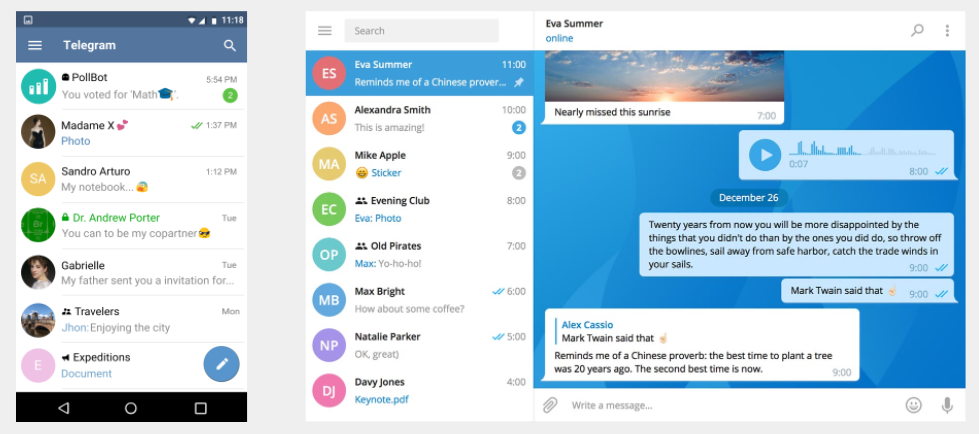
\includegraphics[width=\textwidth]{clients.png}
        \caption{Official Telegram clients. Left: mobile client, right: desktop client. All official Telegram clients are open-source. Telegram provides noticeable faster and smoother user experience.}
        \label{fig:ui-clients}
    \end{figure}
    % mention the command line client and write about it
    
    Telegram even has a command line interface \cite{telegram-cmd}, which provides almost full functionality of the messaging platform albeit it is not as user-friendly. For example, to add a contact one has to write in the interface \\
    \texttt{tg> add\_contact <phone\_number> <name> <lastname>}\\
    We have extensively used the command line interface during this project.
    
    
    
    \section{Telegram Architecture}
   	Like many of its competitors Telegram follows a conventional approach of using a cloud storage for its data. This means that if an adversary is able to gain control of their server system, they will have access to (at least) unencrypted messages and definitely to all the metadata. The messages between users and the server are passed according to Telegram's home-grown MTProto messaging protocol.
    
    The users use a Diffie-Hellman key exchange to generate a common key that is then used to pass messages. They communicate with the server using the server's public RSA key, which is hard-coded in the Telegram clients and changes rarely.
    
    Telegram is using home-grown MTProto protocol, that circumvents many traditional approaches for messaging passing. Telegram claims that this is done for its superior performance, although many security experts have doubts about the claims.
    
    \section{Known and Fixed Security Concerns}
    \label{sec:issues}
    Just like any other tech company, Telegram had, has and will have bugs, security issues and in general security-related issues that are unorthodox in the community. We are presenting some of them here. In next sections we will focus on one of them.
    
    \subsection{Non-technical concerns}
    On a conceptual level, Telegram has some non-standard practices that we believe should not be part of a secure protocol. Namely:
    \begin{itemize}
        \item Telegram's end-to-end encryption feature is not enabled by default on the application \cite{non-encrypted}. For this reason, lots of the users who don't have enough expertise on security/encryption end up using the Telegram without 'secret chat' feature thinking their messages are encrypted. Without secret chats, the users have to trust Telegram servers.
        
        \item Telegram uses a home-grown cryptographic protocol called MTProto, a decision which has been heavily criticized; common security doctrine dictates that developers should never "roll their own" crypto, and should leave cryptographic protocol design to the experts. Those who have examined the protocol themselves have also come away skeptical; cryptographer Matt Green commented that "Telegram is ten million rube goldbergian moving parts, all put there to support a single, unauthenticated Diffie-Hellman key exchange." \cite{mattgreen}
        
        \item Telegram initially asks for the contact list from the phone/desktop and stores them in their servers. This provides huge social network information for them that either be attacked on their servers or can be possibly sold to different authorities without users' consent. This is another case when the users have to trust Telegram with their data.
    \end{itemize}

	\subsection{Technical security issues}
    
    \begin{itemize}
        \item A team of researchers in 2015 announced a man-in-the-middle attack on Telegram that could maybe have been feasible for a nation-state adversary. The attack involves generating Diffie-Hellman shared secrets for the two victims which have the same 128-bit visual fingerprint, so that users who compare fingerprints will be unable to detect the attack; using a birthday attack, this only requires 2\^64 operations. Telegram has since increased the number of fingerprint bits significantly, but the fact that this vulnerability was ever present is still worrying, since it was an error that experts should not make. In order to verify each others' keys and prevent MITM attacks, users must visually compare grids of squares in four shades of blue; this introduces a lot of potential for human error, and users might not notice subtle differences between two grids, or might not be willing to deal with the hassle of comparing the grids in the first place.
        
        \item Until 2014 Telegram's MTProto was using a modified version of a Diffie-Hellman key exchange \cite{habrahabr}. Instead of using the key generated by the usual DH protocol, the server would send the users the key XORed with a \texttt{nonce}. This would allow an evil server to use different \texttt{nonce} variables for the two users. As a result, the users would still have the same key, but it would also be known to the server. Once again, the users had to trust the Telegram server. To their credit Telegram has solved this issue, but just its presence raises questions about their commitment to security, because the issue is a very simple one.

        \item Telegram uses SHA-1 instead of SHA-256 for hashing in some parts of its protocol. It is known that SHA-1 is not collision-resistant \cite{shattered}. Even if Telegram, as it claims, is using SHA-1 at a place where it is not essential to have collision-resistance, using a stronger hash function would be more reasonable. As history has proved many times, bugs and missed cases are common.

        \item Even while using the 'secure chat' to communicate, Telegram's mobile application makes it possible for the third parties to observe the metadata information. For example, adversaries can learn when users go online or offline with down-to-the-second accuracy. Telegram does not require agreement from the both parties to set up the communication between them. For this reason, an attacker might connect to the user and they will receive the metadata information without the user knowing anything about this. For this reason, the attacker might have a good chance of guessing if 2 users communicate by connecting to both of them and observing their app usage metadata. We call this an \textit{availability leak} and will discuss it further in sections \ref{sec:availability} and \ref{sec:results}.
\end{itemize}

    As the previous examples show, in many instances Telegram users should completely trust the server, which is ironic as the founders claim was that they wanted to provide service that is surveillance-proof. Even though many of the security issues were fixed, some of them should not have been there in the first place.
    
    \section{Availability Exploit}
    \label{sec:availability}
    
    As it was briefly mentioned in previous sections, Telegram exposes the users' availability data to anyone who has their phone number. Suppose Eve adds Alice as a contact. The Telegram protocol in this case does not notify Alice about it. Eve, however, gets a response from Telegram whether Alice is using the service, and if so Eve starts receiving notifications about Alice's availability. At no time Alice receives any notification.
    
    \begin{figure}[h!]
    	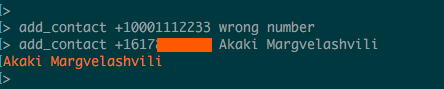
\includegraphics[width=\textwidth]{usage.png}
        \caption{The Telegram CLI outputs the user's name if he/she is using it, but stay silent if not.}
        \label{fig:usage}
    \end{figure}

    This \textit{availability leak} is easily visible in the Telegram command line interface (Telegram CLI). Figure \ref{fig:usage} shows that using the CLI Eve can tell whether Akaki is using the application or no.
    
    \begin{figure}
    	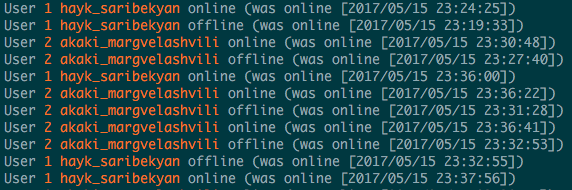
\includegraphics[width=\textwidth]{online-offline.png}
       	\caption{Eve is watching Hayk and Akaki, and can tell when each person becomes available. Notice a bug: the "going offline" times are 5 minutes off.}
        \label{fig:online-offline}
    \end{figure}
    
    Moreover, Figure \ref{fig:online-offline} shows that Eve can see when Akaki and Hayk are becoming available and going offline. She can then correlate the time intervals when both are online and conclude that they converse. In the next sections we describe how exactly this exploit can be used to detect if a pair of users are talking to each other.
    
    \subsection{Experiment Setup}
    We have chosen 15 active Telegram users to track their application usage and communication. The pool of the users were chosen from the well connected international students at MIT. This way we knew that they communicated using telegram on daily/weekly basis.
    
    We have used Telegram command line CLI client to connect to the users. The server has been deployed that was listening for those 15 users' packets and was gathering the metadata for more than 2 weeks. This way, we have gathered several megabytes of the raw metadata to be analyzed.

    \subsection{Correlation Algorithm}
    We have designed a correlation algorithm that takes Telegram usage information of 2 users and outputs a sequence of the matches were each match represents time interval with the probability that users were talking in that time interval (reported probability is always at least 0.5).
    From the gathered metadata, for each user, we created a timeline that shows its activity intervals sorted by time. Algorithm finds matchings of 2 users talking based on their timelines. 
    
    \begin{figure}[!hbt]		
		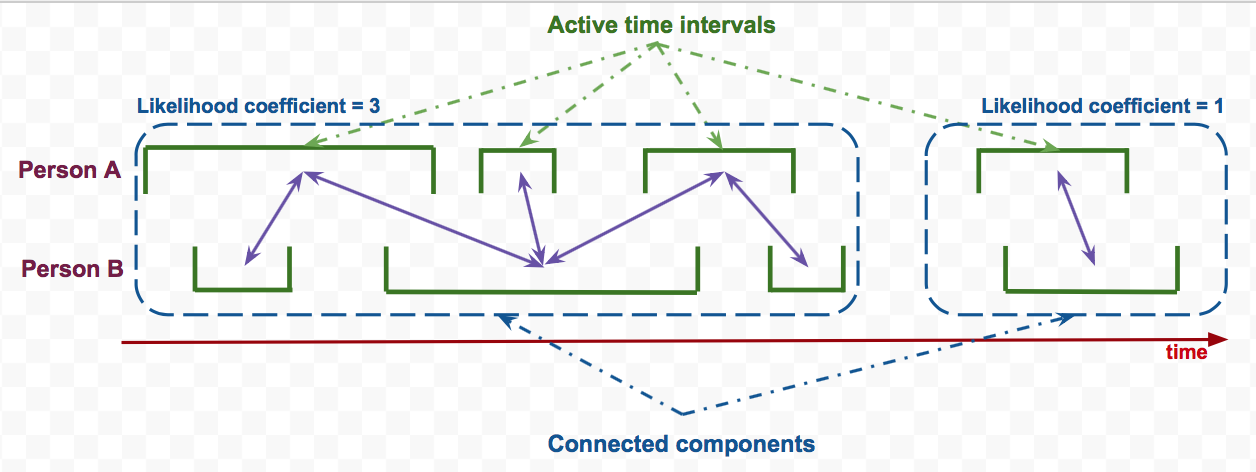
\includegraphics[width=0.99\textwidth]{diagram.png}
		\caption[width=0.5\textwidth]{Diagram illustrating the main concepts of Correlation algorithm.}
		\label{fig:tf_plot}
\end{figure}
    
    We say that active time intervals of Alice and Bob respectively are connected (purple arrow on \textit{Figure 2}) if these time intervals intersect in \textit{gap\_time}. It means that 2 time intervals that have 2 points respectively that are maximum \textit{gap\_time} far away from each other are said to be connected. We do it because, it takes time for the user to open the application after he/she receives a message.
    
      \begin{figure}[h!]		
		\centering
		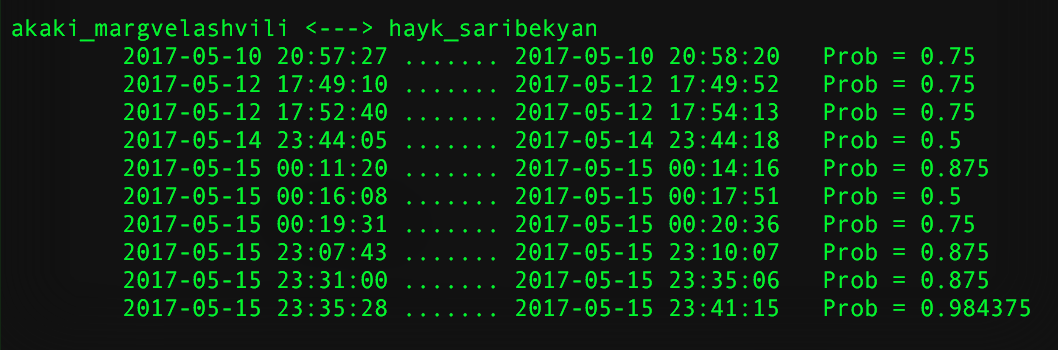
\includegraphics[width=\textwidth]{matches.png}
        \caption{Matchings found by the correlation algorithm.}
        \label{fig:matching}
        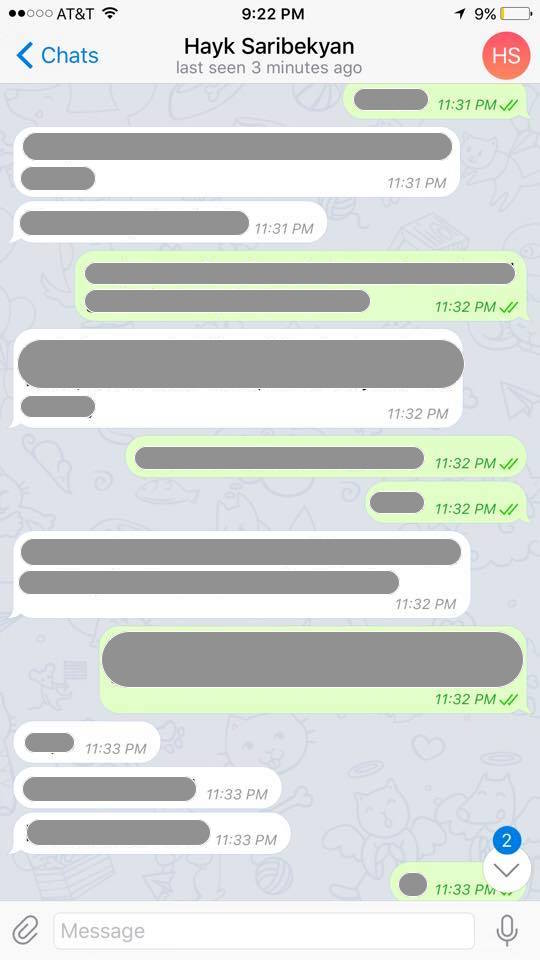
\includegraphics[width=0.5\textwidth]{chat.jpg}
		\caption[width=0.5\textwidth]{Corresponding messages to \ref{fig:matching}. The second to last matching corresponds to the messages in the application (time 23:31 - 23:35)}
		\label{fig:tf_plot1}
\end{figure}
    
    Now, by looking at each of the active time interval as a vertex and each of the connections as an edge we get a \textit{bipartite} graph. In this bipartite graph we look for the \textit{connected components} that has at least 1 edge in it. If we sort the active time intervals in the connected component, we will see the chain of overlapping usages of the Telegram application by Alice and Bob. Every connected pair of time intervals indicates a reasonable probability of the 2 users chatting that time. However, when we have a chain of connected intervals it significantly decreases the chance of Alice and Bob not communicating with each other.
    
    Each connected component represents a separate possible communication (set of messages exchanged in relatively short time of period) between the users. Since the user might leave the Telegram application open (therefore, no metadata information is delivered that time), we do not take into the consideration the size of the active time interval. Rather, we believe that number of the active time intervals is the most important because user going offline and coming online frequently means that he/she is actively engaged in using Telegram.
    
    We define a \textit{likelihood coefficient} to be a measure of how highly likely it is that a connected component represents an actual communication between the users. Note that, an edge in the connected component coming from an active time interval that is connected with many other vertices should be less influential than an edge whose end points are not connected with any other intervals. For this reason, rather than counting number of edges in the connected component, we define \textit{likelihood coefficient} to be one half of all the connected vertexes in the component. This way, a very long active time interval that overlaps lots of other intervals does not increase likelihood coefficient significantly.
    
    Once we calculate a likelihood coefficient, we define a probability of 2 users talking during the span of time in the specific connected component by:
    \[
    P_{texting} = 1 - 2^{-\alpha * coefficient}
    \]
    
    The idea is that if the likelihood coefficient is 0, then $P_{texting} = 0$. However, on every unit added to the coefficient, the probability of not communicating decreases by half. A multiplier $\alpha$ adjusts how smooth or stiff the the influence of the likelihood coefficient should be.
 
  
    \section{Results from Availability Exploit}
    \label{sec:results}
    We implemented the algorithm\footnote{Our code is available at \url{https://github.mit.edu/hayks/857-project}} described above and ran it on the parsed metadata gathered by our server. Since both of us have been using Telegram while the server has been running, we adjusted parameters by looking at our conversations and checking the correctness.
    
    We have found that setting the \textit{gap\_time} to 30 seconds and setting $\alpha = 1$ was giving a reasonable results that was catching all the communications and also was not slicing the actual conversations too much. The results showed that around $15\%$ of all the found matchings were false positives. In other words, sometimes when 2 users happen to use the application at the same time makes an algorithm to be tricked.
    
    
    
    % pretty graphs 
    
    \section{Conclusion}
    \label{sec:conclusion}
    In this project we have surveyed the Telegram messenger. When Telegram has started as a company it became popular because of its claims, public's trust in the founders and also the timing (NSA leaks by Snowden were happened in the same year). Given these claims one would expect very high level of security from Telegram. However, our survey shows that Telegram has had serious and simple issues in the protocol (e.g. modified buggy Diffie-Hellman key exchange) that any knowledgeable security expert could penetrate.

	By using the command line interface of Telegram we have been able to snoop on some of our friends and detect the times when they were conversing to each other. We believe that this is a serious privacy issue, because it can be exploited to detect relationships in classroom for example.
    
    Finally, our conclusion is that Telegram, just like any other application has vulnerabilities. Users have to be aware of this fact, but unfortunately the claims by companies make non-tech-savvy users to believe that their messages are unreadable by third parties.
    
    \bibliographystyle{unsrt}
    \bibliography{references}

\end{document}
